\documentclass[12pt, a4paper]{article}

\usepackage[utf8]{inputenc}
\usepackage[T5]{fontenc}
\usepackage[vietnamese]{babel}
\usepackage{amsmath, amssymb}
\usepackage{graphicx}
\usepackage{geometry}
\usepackage{hyperref}
\usepackage{fancyhdr}
\usepackage{tocloft}
\usepackage{titlesec}
\usepackage{caption}
\usepackage{subcaption}
\usepackage{float}
\usepackage{tikz}
\usepackage{multirow}
\usepackage{listings}
\usepackage[table]{xcolor}
\usetikzlibrary{calc}

\geometry{
    a4paper,
    total={170mm,257mm},
    left=30mm,
    right=20mm,
    top=20mm,
    bottom=20mm,
}

\begin{document}
\begin{titlepage}
    \begin{tikzpicture}[remember picture, overlay]
        \draw[color=cyan!70!blue, line width = 2pt] 
            ($(current page.north west) + (2cm,-1.5cm)$) 
            rectangle 
            ($(current page.south east) + (-1.5cm,1.5cm)$);
        \draw[color=cyan!70!blue, line width = 0.5pt] 
            ($(current page.north west) + (2.1cm,-1.6cm)$) 
            rectangle 
            ($(current page.south east) + (-1.6cm,1.6cm)$);
    \end{tikzpicture}

    \begin{center}
        \vspace*{0.5cm}
        \textbf{\large BỘ GIÁO DỤC VÀ ĐÀO TẠO} \\[0.2cm]
        \textbf{\Large TRƯỜNG ĐẠI HỌC SÀI GÒN} \\[0.2cm]
        \textbf{\large KHOA TOÁN - ỨNG DỤNG} \\[1cm]

        
\includegraphics[width=6cm]{logo.png} \\[0.5cm] 
        
        \vspace{0.5cm}
        \textbf{\Large BÁO CÁO ĐỒ ÁN} \\[0.5cm]
        \textbf{\Large NGHIÊN CỨU THUẬT TOÁN ĐÀN MÒNG BIỂN} \\[0.2cm]
        \textbf{\Large ĐA CHIẾN LƯỢC (MISOA) VÀ ỨNG DỤNG} \\[0.2cm]
        \textbf{\Large TRONG TỐI ƯU HÓA ĐƯỜNG ĐI} \\[0.5cm]
        \textbf{\large Học phần: Cơ Sở Trí Tuệ Nhân Tạo} \\[1cm]

        \begin{flushleft}
            \large
            \hspace{1.5cm} \textbf{Giảng viên hướng dẫn:} Huỳnh Minh Trí \\[0.5cm]
            \hspace{1.5cm} \textbf{Sinh viên thực hiện:} \\[0.2cm]
            \hspace{2.5cm} 1. Nguyễn Trương Cao Sơn \hspace{0.5cm} MSSV: 3123580040 \\[0.2cm]
            \hspace{2.5cm} 2. Phan Đồng Minh Quân \hspace{0.75cm} MSSV: 3123580038 \\[0.2cm]
            \hspace{2.5cm} 3. Võ Minh Tiến \hspace{2.3cm} MSSV: 3123580053 \\[0.5cm]
        \end{flushleft}

        \vfill
        {\large TP Hồ Chí Minh, năm 2026}
        \vspace*{0.5cm}
    \end{center}
\end{titlepage}

% ====================================================
% PHẦN MỞ ĐẦU & DANH MỤC
% ====================================================
\newpage
\phantomsection
\section*{LỜI CẢM ƠN}
\addcontentsline{toc}{section}{Lời cảm ơn}
Nhóm chúng em xin gửi lời cảm ơn chân thành và sâu sắc nhất đến Thầy \textbf{Huỳnh Minh Trí} — giảng viên phụ trách môn \textit{Cơ sở trí tuệ nhân tạo}.

Trong suốt thời gian thực hiện đồ án, Thầy đã luôn tận tâm hướng dẫn, định hướng nghiên cứu và đưa ra những góp ý chuyên môn vô cùng quý giá. Những chỉ dẫn của Thầy không chỉ giúp nhóm tháo gỡ các nút thắt về thuật toán tối ưu hóa Metaheuristic mà còn giúp chúng em rèn luyện tư duy lập trình và phương pháp trình bày báo cáo khoa học chuẩn mực.

Mặc dù đã nỗ lực hết sức để hoàn thiện đồ án với đề tài \textit{"Nghiên cứu và cải tiến thuật toán tối ưu hóa đàn mòng biển đa chiến lược (MISOA)"}, nhưng do giới hạn về mặt thời gian cũng như kinh nghiệm thực tiễn, báo cáo chắc chắn vẫn còn tồn tại những thiếu sót nhất định.

Nhóm kính mong nhận được sự thông cảm, cùng những lời nhận xét, đánh giá phản biện từ Thầy để đồ án được hoàn thiện hơn, đồng thời mở ra các hướng ứng dụng thực tế trong tương lai. Một lần nữa, chúng em xin kính chúc Thầy dồi dào sức khỏe, thành công trong sự nghiệp giảng dạy và nghiên cứu khoa học.

Chúng em xin chân thành cảm ơn!

\vspace{1cm}
\begin{flushright}
\textit{TP. Hồ Chí Minh, năm 2026} \\
\textbf{Nhóm thực hiện} \\
\vspace{0.2cm}
Nguyễn Trương Cao Sơn \\
Phan Đồng Minh Quân \\
Võ Minh Tiến
\end{flushright}

\newpage
\phantomsection
\section*{ABSTRACT}
\addcontentsline{toc}{section}{Abstract}

\begin{quotation}
\noindent
Trong bối cảnh ngành vận tải và hậu cần đang ngày càng chú trọng vào tối ưu hóa chi phí, bài toán định tuyến đường đi đóng vai trò quyết định trong việc nâng cao hiệu quả chuỗi cung ứng. Đồ án nghiên cứu và đề xuất thuật toán Đàn mòng biển cải tiến đa chiến lược (MISOA) nhằm khắc phục hạn chế về tốc độ hội tụ và khả năng thoát bẫy cục bộ của thuật toán Đàn mòng biển (SOA) nguyên bản.

Nghiên cứu thực hiện ba cải tiến: (1) Áp dụng Ánh xạ hỗn mang Logistic để khởi tạo quần thể; (2) Thiết kế biến kiểm soát phi tuyến tính dựa trên hàm bậc hai; (3) Tích hợp cơ chế đột biến Bước nhảy Levy. 

Kết quả thực nghiệm trên các hàm kiểm thử tiêu chuẩn cho thấy MISOA đạt độ chính xác vượt trội hơn nhiều lần so với SOA gốc. Đặc biệt, tại hàm đa cực trị F9, MISOA là thuật toán duy nhất tìm được giá trị tối ưu tuyệt đối bằng 0. \textbf{Tuy nhiên, kết quả cũng ghi nhận sự đánh đổi về tính ổn định trên một số không gian tìm kiếm phức tạp, nơi đặc tính đột biến mạnh của Bước nhảy Levy giúp tìm ra nghiệm tối ưu cực hạn nhưng đồng thời làm gia tăng độ lệch chuẩn của tập nghiệm.} Cuối cùng, nhóm triển khai ứng dụng thực tiễn trên nền tảng Web thông qua Streamlit, giúp tối ưu hóa lộ trình giao hàng và tiết kiệm chi phí nhiên liệu thực tế.
\end{quotation}

\vspace{0.5cm}
\noindent
\textbf{Từ khóa:} Thuật toán tối ưu hóa Đàn mòng biển, MISOA, Bước nhảy Levy, Ánh xạ hỗn mang, Tối ưu hóa định tuyến.

\newpage
\tableofcontents

\newpage
\phantomsection
\addcontentsline{toc}{section}{Danh mục hình ảnh}
\listoffigures

\newpage
\phantomsection
\addcontentsline{toc}{section}{Danh mục bảng biểu}
\listoftables

\newpage
\phantomsection
\section*{DANH MỤC TỪ VIẾT TẮT}
\addcontentsline{toc}{section}{Danh mục từ viết tắt}
\begin{itemize}
    \item \textbf{SOA}: Seagull Optimization Algorithm (Thuật toán tối ưu hóa đàn mòng biển)
    \item \textbf{MISOA}: Multi-strategy Improved Seagull Optimization Algorithm (Thuật toán đàn mòng biển cải tiến đa chiến lược)
    \item \textbf{TSP} \> Bài toán Người giao hàng (Traveling Salesman Problem)
    \item \textbf{VRP} \> Bài toán Định tuyến phương tiện (Vehicle Routing Problem)
    \item \textbf{ROV} \> Giá trị thứ tự xếp hạng (Rank Order Value)
    \item \textbf{NFL} \> Định lý Không có bữa trưa miễn phí (No Free Lunch Theorem)
    \item \textbf{AI} \> Trí tuệ nhân tạo (Artificial Intelligence)
    \item \textbf{NP-Hard} \> Bài toán khó đa thức không xác định (Non-deterministic Polynomial-time Hard)
    \item \textbf{MAKL} \> Ánh xạ hỗn mang Logistic (Chaotic Logistic Map)
    \item \textbf{UI/UX} \> Giao diện và Trải nghiệm người dùng (User Interface/User Experience)
\end{itemize}

% ====================================================
% NỘI DUNG CHÍNH (CÁC CHƯƠNG)
% ====================================================
\newpage
\pagenumbering{arabic}

% ---------- CHƯƠNG 1 ----------
\newpage
\section{TỔNG QUAN VỀ ĐỀ TÀI VÀ BÀI TOÁN TỐI ƯU HÓA}

\subsection{Bối cảnh nghiên cứu và Lý do chọn đề tài}
Trong kỷ nguyên công nghiệp 4.0, logistics và vận tải đóng vai trò xương sống trong nền kinh tế toàn cầu. Sự bùng nổ của thương mại điện tử đặt ra thách thức lớn về việc tối ưu hóa quy trình phân phối hàng hóa nhằm giảm thiểu chi phí vận hành và thời gian giao hàng. Bài toán định tuyến, cụ thể là tìm kiếm lộ trình ngắn nhất đi qua các điểm giao hàng, là một bài toán tối ưu hóa tổ hợp kinh điển thuộc lớp NP-Hard với nhiều nghiên cứu sâu rộng \cite{tsp_survey}. Việc giải quyết bài toán này bằng các phương pháp toán học truyền thống gặp nhiều hạn chế khi quy mô dữ liệu tăng lên. Do đó, ứng dụng các thuật toán siêu cảm hứng (Metaheuristic) đang trở thành xu hướng tất yếu nhờ khả năng tìm kiếm nghiệm xấp xỉ tối ưu trong thời gian chấp nhận được.

\subsection{Vấn đề nghiên cứu}
Thuật toán tối ưu hóa Đàn mòng biển (SOA) được đề xuất bởi Dhiman và Kumar \cite{soa_original} là một thuật toán tối ưu hóa mới dựa trên đặc tính di cư và săn mồi của loài chim này. Tuy nhiên, SOA nguyên bản thường đối mặt với các vấn đề về tốc độ hội tụ chậm và dễ rơi vào các bẫy cực tiểu cục bộ khi giải quyết các hàm mục tiêu đa cực trị hoặc bài toán tổ hợp phức tạp. Nghiên cứu này tập trung vào việc cải tiến các cơ chế vận động của SOA nhằm nâng cao hiệu suất tìm kiếm nghiệm.

\subsection{Mục tiêu và Phạm vi nghiên cứu}
\textbf{Mục tiêu:} Đề xuất thuật toán MISOA bằng cách tích hợp ánh xạ hỗn mang, biến kiểm soát phi tuyến tính và bước nhảy Levy. Đồng thời, xây dựng ứng dụng thực tiễn để giải quyết bài toán định tuyến đường đi. \\
\textbf{Phạm vi:} Nghiên cứu giới hạn trong việc cải tiến thuật toán SOA trên không gian liên tục và rời rạc (thông qua kỹ thuật ROV), thực nghiệm trên bộ hàm kiểm thử tiêu chuẩn và ứng dụng vào bài toán định tuyến quy mô vừa và nhỏ.

\subsection{Câu hỏi nghiên cứu}
\begin{itemize}
    \item Thuật toán SOA nguyên bản gặp những hạn chế cụ thể nào khi giải các bài toán tối ưu hóa phức tạp?
    \item Việc kết hợp đa chiến lược có thực sự cải thiện khả năng thoát bẫy cục bộ của thuật toán?
    \item Hiệu quả kinh tế thực tiễn khi ứng dụng thuật toán vào bài toán định tuyến đường đi là bao nhiêu?
\end{itemize}

\subsection{Các giải pháp tương đương}
Hiện nay, có nhiều thuật toán đã được ứng dụng thành công cho bài toán định tuyến như: Thuật toán Di truyền (GA), Tối ưu hóa bầy đàn (PSO) và Tối ưu hóa thuộc địa kiến (ACO). So với các giải pháp này, MISOA hướng tới việc cân bằng tốt hơn giữa khả năng khám phá không gian và khai thác nghiệm cục bộ, đồng thời giảm thiểu độ phức tạp về mặt tham số cấu hình.

\subsection{Ý nghĩa khoa học và Thực tiễn}
\textbf{Về khoa học:} Đóng góp một biến thể mới cho họ thuật toán siêu cảm hứng, làm phong phú thêm các phương pháp tối ưu hóa hiện đại. \\
\textbf{Về thực tiễn:} Cung cấp một công cụ hỗ trợ ra quyết định cho các đơn vị vận chuyển, giúp tiết kiệm chi phí nhiên liệu, giảm lượng khí thải và tối ưu hóa tài nguyên doanh nghiệp.

\subsection{Cấu trúc của báo cáo}
Nội dung của đồ án được trình bày logic thông qua 6 chương chính, cụ thể như sau:
\begin{itemize}
    \item \textbf{Chương 1 - Tổng quan về đề tài và bài toán tối ưu hóa:} Giới thiệu bối cảnh, mục tiêu và ý nghĩa của đề tài.
    \item \textbf{Chương 2 - Cơ sở lý thuyết về thuật toán Đàn mòng biển:} Trình bày chi tiết mô hình toán học cho thuật toán nguyên bản.
    \item \textbf{Chương 3 - Đề xuất cải tiến thuật toán đa chiến lược (MISOA):} Phân tích hạn chế của thuật toán gốc và trình bày ba chiến lược cải tiến chủ chốt.
    \item \textbf{Chương 4 - Thực nghiệm đánh giá trên bộ hàm kiểm thử toán học:} Đánh giá thống kê hiệu suất giữa SOA và MISOA.
    \item \textbf{Chương 5 - Triển khai ứng dụng thực tiễn và giao diện tương tác:} Ứng dụng thuật toán vào bài toán giao hàng thực tế.
    \item \textbf{Chương 6 - Kết luận và hướng phát triển:} Tổng kết, thừa nhận hạn chế và đề xuất nghiên cứu tương lai.
\end{itemize}

% ---------- CHƯƠNG 2 ----------
\newpage
\section{CƠ SỞ LÝ THUYẾT VỀ THUẬT TOÁN ĐÀN MÒNG BIỂN}

\subsection{Nguồn cảm hứng sinh học}
Thuật toán tối ưu hóa Đàn mòng biển \cite{soa_original} mô phỏng các hành vi sinh tồn đặc trưng của loài chim này trong tự nhiên, bao gồm sự di cư của bầy đàn và hành vi tấn công con mồi theo hình xoắn ốc. Trong quá trình di cư, các cá thể duy trì vị trí để tránh va chạm. Khi săn mồi, chúng thay đổi độ cao và góc độ để tấn công theo quỹ đạo xoắn ốc độc đáo.

\begin{itemize}
    \item \textbf{Hành vi di cư:} Đàn mòng biển di chuyển từ vị trí này sang vị trí khác để tìm kiếm nguồn thức ăn dồi dào hơn. Trong quá trình này, các cá thể phải đảm bảo không va chạm với nhau và luôn hướng về phía cá thể có vị trí tốt nhất.
    \item \textbf{Hành vi săn mồi:} Khi phát hiện mục tiêu, mòng biển thực hiện các chuyển động theo quỹ đạo xoắn ốc để tấn công con mồi một cách chính xác. 
\end{itemize}

\subsection{Mô hình hóa toán học giai đoạn di cư}
Trong giai đoạn này, thuật toán thực hiện việc khám phá không gian tìm kiếm. Mô hình được xây dựng dựa trên ba quy tắc chính:

\subsubsection{Tránh va chạm}
Để tránh va chạm giữa các cá thể lân cận, một biến bổ sung $A$ được sử dụng để cập nhật vị trí của cá thể mòng biển:
\begin{equation}
    \vec{C_s} = A \times \vec{P_s}(t)
\end{equation}
Trong đó:
\begin{itemize}
    \item $\vec{C_s}$ là vị trí mới không gây va chạm.
    \item $\vec{P_s}(t)$ là vị trí hiện tại của cá thể ở vòng lặp $t$.
    \item $A$ là hệ số di chuyển của mòng biển, được tính theo công thức: $A = f_c - (t \times (f_c / Max_{iter}))$, với $f_c$ là tần số kiểm soát (thường mặc định bằng 2).
\end{itemize}

\subsubsection{Di chuyển về phía cá thể tốt nhất}
Sau khi đảm bảo không va chạm, các cá thể sẽ di chuyển về hướng của cá thể có độ thích nghi tốt nhất trong quần thể:
\begin{equation}
    \vec{M_s} = B \times (\vec{P_{best}}(t) - \vec{P_s}(t))
\end{equation}
Trong đó:
\begin{itemize}
    \item $\vec{M_s}$ đại diện cho hướng di chuyển về phía cá thể tốt nhất.
    \item $\vec{P_{best}}(t)$ là vị trí của cá thể tốt nhất tại vòng lặp $t$.
    \item $B$ là hệ số ngẫu nhiên giúp cân bằng quá trình khám phá, được tính bằng: $B = 2 \times r^2$ với $r$ là số ngẫu nhiên trong khoảng $[0, 1]$.
\end{itemize}

\subsubsection{Khoảng cách gần với cá thể tốt nhất}
Cuối cùng, vị trí của mòng biển được cập nhật sao cho nó duy trì khoảng cách tối ưu với vị trí tốt nhất:
\begin{equation}
    \vec{D_s} = |\vec{C_s} + \vec{M_s}|
\end{equation}

\subsection{Mô hình hóa toán học giai đoạn tấn công}
Giai đoạn này mô phỏng quá trình khai thác cục bộ nghiệm. Mòng biển tấn công con mồi theo quỹ đạo xoắn ốc trong không gian ba chiều. Các tọa độ chuyển động được xác định như sau:
\begin{equation}
    x = r \times \cos(k)
\end{equation}
\begin{equation}
    y = r \times \sin(k)
\end{equation}
\begin{equation}
    z = r \times k
\end{equation}
\begin{equation}
    r = u \times e^{kv}
\end{equation}
Trong đó:
\begin{itemize}
    \item $r$ là bán kính của vòng xoắn ốc.
    \item $k$ là biến ngẫu nhiên trong khoảng $[0, 2\pi]$.
    \item $u$ và $v$ là các hằng số xác định hình dạng đường xoắn ốc.
\end{itemize}
Vị trí cập nhật cuối cùng của mòng biển được tính theo công thức:
\begin{equation}
    \vec{P_s}(t) = (\vec{D_s} \times x \times y \times z) + \vec{P_{best}}(t)
\end{equation}
Sự kết hợp giữa di chuyển tuyến tính trong di cư và di chuyển phi tuyến trong tấn công giúp thuật toán có khả năng bao phủ không gian tìm kiếm rộng lớn trước khi tập trung vào vùng nghiệm tiềm năng.

% ---------- CHƯƠNG 3 ----------
\newpage
\section{ĐỀ XUẤT CẢI TIẾN THUẬT TOÁN ĐA CHIẾN LƯỢC (MISOA)}

\subsection{Hạn chế của thuật toán cơ sở và vấn đề hội tụ cục bộ}
Mặc dù thuật toán đàn mòng biển nguyên bản (SOA) cho thấy hiệu năng tốt trên các bài toán tối ưu hóa cơ bản, nó vẫn tồn tại ba nhược điểm lớn khi đối mặt với các không gian tìm kiếm phức tạp (đa mode):
\begin{enumerate}
    \item \textbf{Khởi tạo ngẫu nhiên thiếu đồng đều:} Việc sử dụng phân phối ngẫu nhiên thuần túy khiến quần thể ban đầu dễ bị co cụm tại một khu vực, làm giảm khả năng bao quát không gian.
    \item \textbf{Mất cân bằng giữa Khám phá và Khai thác:} Tham số kiểm soát $Fc$ giảm tuyến tính khiến thuật toán chuyển đổi trạng thái một cách cứng nhắc, không đủ thời gian để rà soát các vùng tiềm năng ở giai đoạn đầu.
    \item \textbf{Dễ hội tụ sớm:} Khi gặp các hàm có nhiều cực tiểu cục bộ như hàm Rastrigin, toàn bộ đàn mòng biển dễ bị mắc kẹt tại một hố cạn và không có cơ chế đột biến đủ mạnh để thoát ra.
\end{enumerate}
Để khắc phục triệt để các hạn chế này, đồ án đề xuất phiên bản cải tiến MISOA với sự tích hợp của ba chiến lược toán học tiên tiến.

\subsection{Cải tiến khởi tạo quần thể dựa trên ánh xạ hỗn mang}
Thay vì sử dụng các hàm sinh số ngẫu nhiên truyền thống, MISOA áp dụng ánh xạ hỗn mang \cite{chaotic_maps} Logistic để phân bố đàn mòng biển. Đặc tính ergodic và không lặp lại của hệ thống hỗn mang giúp các cá thể trải đều khắp không gian tìm kiếm, tăng xác suất tìm thấy vùng chứa nghiệm tối ưu toàn cục ngay từ vòng lặp đầu tiên.

Phương trình cập nhật của Logistic Map được định nghĩa như sau:
\begin{equation}
x_{n+1} = a \cdot x_n \cdot (1 - x_n)
\end{equation}
Trong đó, $x_n$ là giá trị hỗn mang ở bước $n$, và $a = 4.0$ là tham số kiểm soát để hệ thống đạt trạng thái hỗn loạn cực đại. Quần thể sau khi trải qua quá trình hỗn mang sẽ được ánh xạ ngược trở lại không gian tìm kiếm thực tế thông qua các giới hạn trên và dưới của bài toán.

\subsection{Tối ưu hóa tham số kiểm soát theo phương pháp phi tuyến tính}
Để giải quyết sự cứng nhắc của hàm tuyến tính trong SOA nguyên bản, MISOA đề xuất sử dụng hàm suy giảm phi tuyến tính dạng Parabol ngược cho tham số $Fc$. Cấu trúc này giúp đàn mòng biển duy trì trạng thái bay lượn ngó nghiêng hây gọi là Exploration lâu hơn ở nửa đầu thời gian, và cắm dốc cực nhanh ở nửa sau để chốt hạ mục tiêu tức là Exploitation.

Công thức cập nhật biến $Fc$ cải tiến được biểu diễn bằng phương trình:
\begin{equation}
Fc = 2 \cdot \left(1 - \frac{l}{Max\_iter}\right)^2
\end{equation}
Trong đó, $l$ là vòng lặp hiện tại và $Max\_iter$ là tổng số vòng lặp tối đa. Việc bình phương tỷ lệ thời gian đảm bảo thuật toán không bị rơi tự do quá sớm, cải thiện đáng kể độ chính xác.

\subsection{Ứng dụng chiến thuật bước nhảy Levy thoát khỏi cực tiểu cục bộ}
Để trị dứt điểm căn bệnh "kẹt cực tiểu cục bộ", chiến thuật Bước nhảy Levy \cite{levy_flight} được áp dụng như một cơ chế đột biến. Tuy nhiên, việc áp dụng Levy mù quáng có thể phá vỡ sự hội tụ ở những vòng lặp cuối. Do đó, MISOA sử dụng \textbf{Levy Flight Thích nghi} kết hợp cùng \textbf{Cơ chế chọn lọc tham lam}.

Thuật toán cấp phát một xác suất nhỏ ($20\%$) để mòng biển thực hiện đột biến vị trí dựa trên công thức:
\begin{equation}
X_{new} = X_{current} + \alpha \cdot Levy(d) \cdot \left(1 - \frac{l}{Max\_iter}\right)^2
\end{equation}

\textbf{Phân tích logic của chiến lược:}
\begin{itemize}
    \item \textbf{Hệ số suy giảm:} Cụm $\left(1 - \frac{l}{Max\_iter}\right)^2$ đóng vai trò như một "khóa an toàn". Ở các vòng lặp đầu, lực nhảy mạnh giúp mòng biển văng xa khỏi các bẫy cục bộ. Càng về cuối, lực nhảy bị triệt tiêu dần về 0.
    \item \textbf{Chọn lọc tham lam:} Vị trí mới $X_{new}$ chỉ được chấp nhận nếu giá trị độ thích nghi của nó tốt hơn vị trí hiện tại. Điều này đảm bảo thuật toán luôn tiến lên phía trước.
\end{itemize}

\subsection{Lưu đồ thuật toán cải tiến đề xuất}

Để mang lại cái nhìn tổng thể về sự kết hợp giữa các chiến lược cải tiến, lưu đồ thuật toán MISOA được xây dựng nhằm minh chứng cho quy trình vận hành chặt chẽ từ khâu khởi tạo hỗn mang đến khâu đột biến bước nhảy Levy.

\subsubsection{Mô tả các bước vận hành}
Quy trình thực hiện được chuẩn hóa thành 6 giai đoạn chính tương ứng với lưu đồ Hình \ref{fig:misoa_flowchart}:
\begin{itemize}
    \item \textbf{Bước 1: Khởi tạo.} Thiết lập tham số ($N, D, Max_{iter}$) và khởi tạo quần thể bằng Ánh xạ hỗn mang để đảm bảo tính phân tán toàn cục.
    \item \textbf{Bước 2: Đánh giá thích nghi.} Tính giá trị hàm mục tiêu và xác định cá thể tốt nhất $\vec{P_{best}}$ làm mục tiêu tấn công cho cả đàn.
    \item \textbf{Bước 3: Cập nhật tham số kiểm soát.} Tính toán biến $Fc$ theo hàm bậc hai giảm dần để điều phối sự cân bằng giữa Khám phá và Khai thác.
    \item \textbf{Bước 4: Cập nhật vị trí di cư và tấn công.} Áp dụng đồng thời cơ chế tránh va chạm tuyến tính và tấn công xoắn ốc phi tuyến hướng tâm.
    \item \textbf{Bước 5: Đột biến Levy Flight.} Thực hiện các cú nhảy ngẫu nhiên dài để giúp cá thể văng khỏi các bẫy cực tiểu cục bộ.
    \item \textbf{Bước 6: Kết xuất kết quả.} Kiểm tra điều kiện dừng và xuất ra nghiệm tối ưu nhất sau khi thuật toán hội tụ.
\end{itemize}

\subsubsection{Lưu đồ thuật toán tổng quát}
Dưới đây là lưu đồ mô tả chi tiết luồng xử lý của thuật toán MISOA:

\begin{figure}[H]
    \centering
    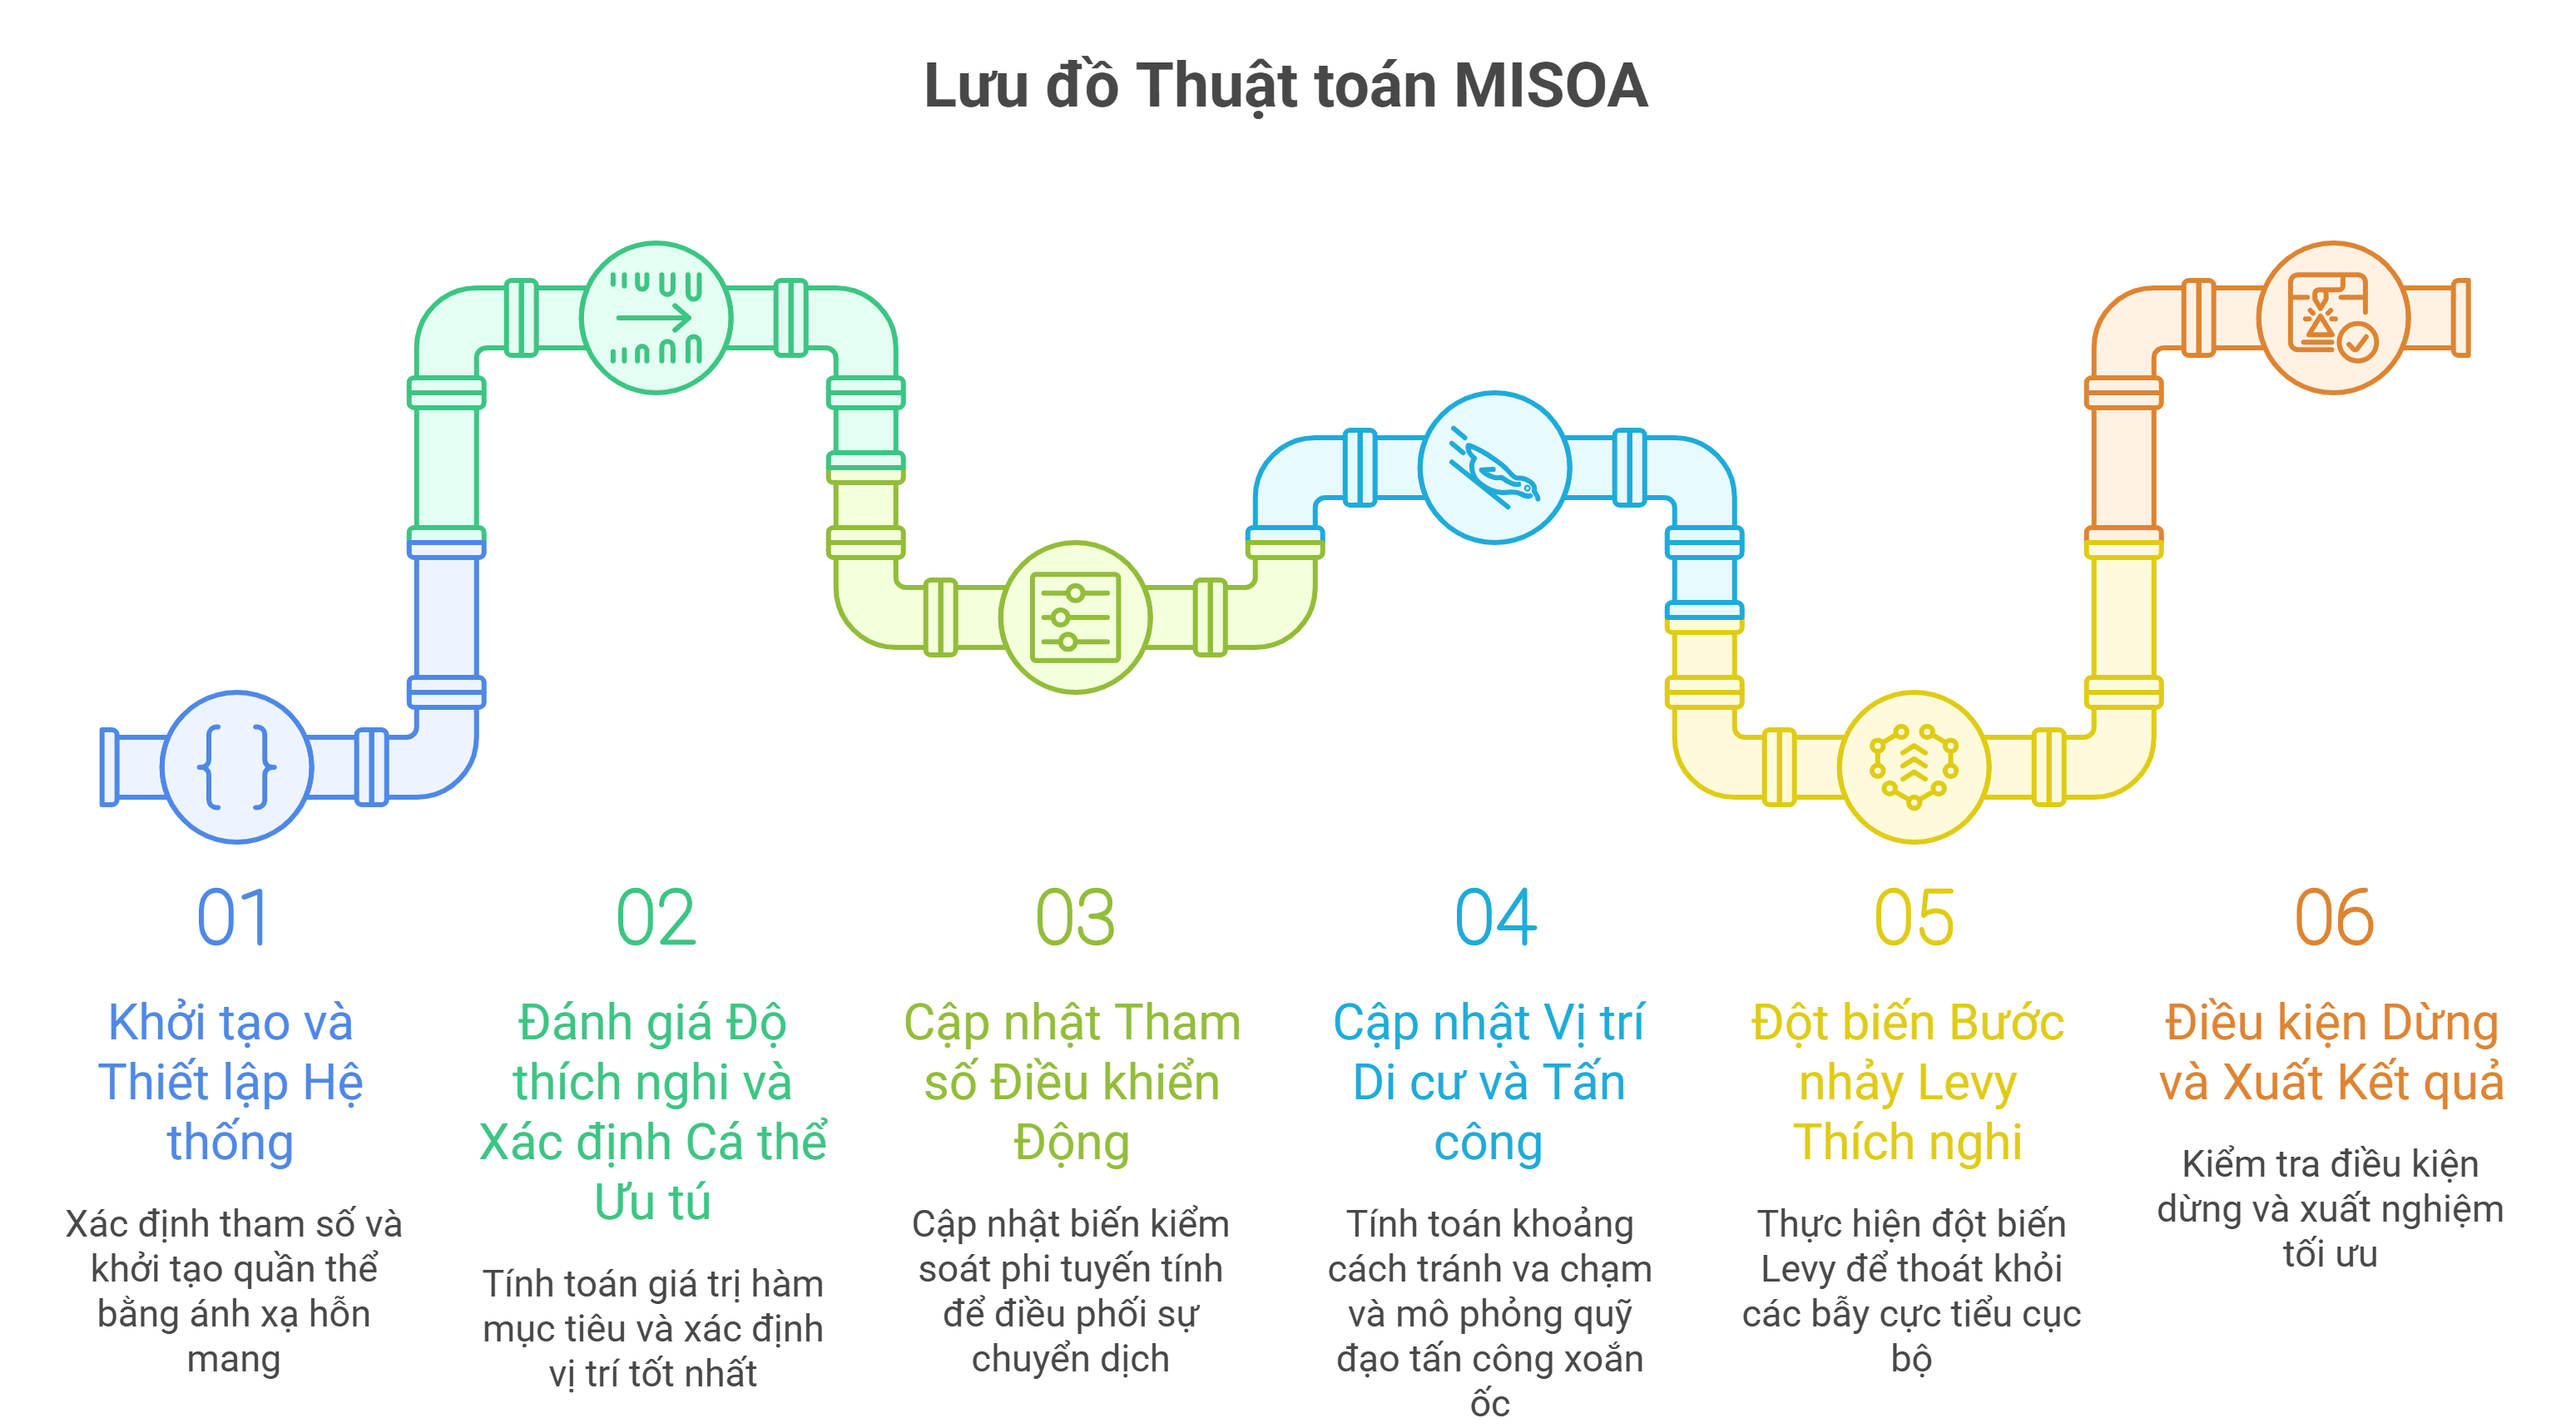
\includegraphics[width=0.8\textwidth]{images/misoa_flowchart.png}
    \caption{Lưu đồ thuật toán Đàn mòng biển cải tiến đa chiến lược (MISOA)}
    \label{fig:misoa_flowchart}
\end{figure}

Việc thiết lập lưu đồ như trên cho thấy sự cải tiến của MISOA không làm thay đổi cấu trúc đơn giản, hiệu quả của thuật toán SOA nguyên bản, mà chỉ tập trung nâng cấp "chất lượng" di chuyển của các cá thể thông qua các toán tử thông minh. Điều này đảm bảo thuật toán vẫn duy trì được tốc độ xử lý nhanh trong khi độ chính xác được cải thiện rõ rệt.

% ---------- CHƯƠNG 4 ----------
\newpage
\section{THỰC NGHIỆM ĐÁNH GIÁ TRÊN BỘ HÀM KIỂM THỬ TOÁN HỌC}

\subsection{Môi trường cài đặt và cấu hình tham số hệ thống}
Để đảm bảo tính công bằng và minh bạch trong quá trình so sánh, toàn bộ các thực nghiệm được lập trình bằng ngôn ngữ Python (phiên bản 3.x) kết hợp với các thư viện tính toán khoa học Numpy và Pandas. Thực nghiệm được tiến hành trên nền tảng phần cứng máy tính Gigabyte G5.

Các tham số hệ thống cấu hình chung cho cả hai thuật toán (SOA và MISOA) được thiết lập theo tiêu chuẩn nghiên cứu Metaheuristic quốc tế nhằm đảm bảo tính ổn định của thống kê:
\begin{itemize}
    \item Số lượng cá thể mòng biển: $N = 30$
    \item Số chiều không gian tìm kiếm: $D = 30$
    \item Tổng số vòng lặp tối đa: $Max\_iter = 500$
    \item Số lần chạy độc lập: $Runs = 30$
\end{itemize}

\subsection{Xây dựng bộ hàm kiểm thử tiêu chuẩn}
Hệ thống sử dụng 4 hàm kiểm thử kinh điển chia làm hai nhóm chính để đánh giá toàn diện năng lực của thuật toán:

\textbf{1. Nhóm hàm đơn mode:} Đánh giá tốc độ hội tụ và khả năng khai thác độ chính xác sâu.
\begin{itemize}
    \item \textbf{F1 (Sphere):} $f_1(x) = \sum_{i=1}^{D} x_i^2$ \\
    Không gian: $[-100, 100]^D$. Giá trị tối ưu: $f(x^*) = 0$.
    \item \textbf{F2 (Schwefel 2.22):} $f_2(x) = \sum_{i=1}^{D} |x_i| + \prod_{i=1}^{D} |x_i|$ \\
    Không gian: $[-10, 10]^D$. Giá trị tối ưu: $f(x^*) = 0$.
\end{itemize}

\textbf{2. Nhóm hàm đa mode:} Đánh giá khả năng khám phá và thoát khỏi bẫy cực tiểu cục bộ.
\begin{itemize}
    \item \textbf{F9 (Rastrigin):} $f_9(x) = \sum_{i=1}^{D} \left[ x_i^2 - 10 \cos(2\pi x_i) + 10 \right]$ \\
    Không gian: $[-5.12, 5.12]^D$. Giá trị tối ưu: $f(x^*) = 0$.
    \item \textbf{F10 (Ackley):} $f_{10}(x) = -20 \exp\left(-0.2 \sqrt{\frac{1}{D}\sum_{i=1}^{D} x_i^2}\right) - \exp\left(\frac{1}{D}\sum_{i=1}^{D} \cos(2\pi x_i)\right) + 20 + e$ \\
    Không gian: $[-32.768, 32.768]^D$. Giá trị tối ưu: $f(x^*) = 0$.
\end{itemize}

\subsection{Đánh giá trực quan thông qua đường cong hội tụ}
Để chứng minh tính hiệu quả và độ ổn định của thuật toán Đàn mòng biển cải tiến đa chiến lược (MISOA), hệ thống đã tiến hành thực nghiệm trên tập các hàm kiểm thử tiêu chuẩn bao gồm nhóm hàm đơn cực trị và đa cực trị. Các đường cong hội tụ được kết xuất trực tiếp từ quá trình thực thi mã nguồn nhằm phản ánh chính xác tốc độ hội tụ và năng lực thoát khỏi các vùng tối ưu cục bộ của thuật toán.

\textbf{Đánh giá năng lực khai thác trên không gian đơn cực trị (F1, F2)}

Hàm F1 đóng vai trò là bài toán kiểm thử cơ bản để xác định khả năng tăng tốc hội tụ của thuật toán cải tiến trong các không gian lồi đơn giản.

\begin{figure}[H]
    \centering
    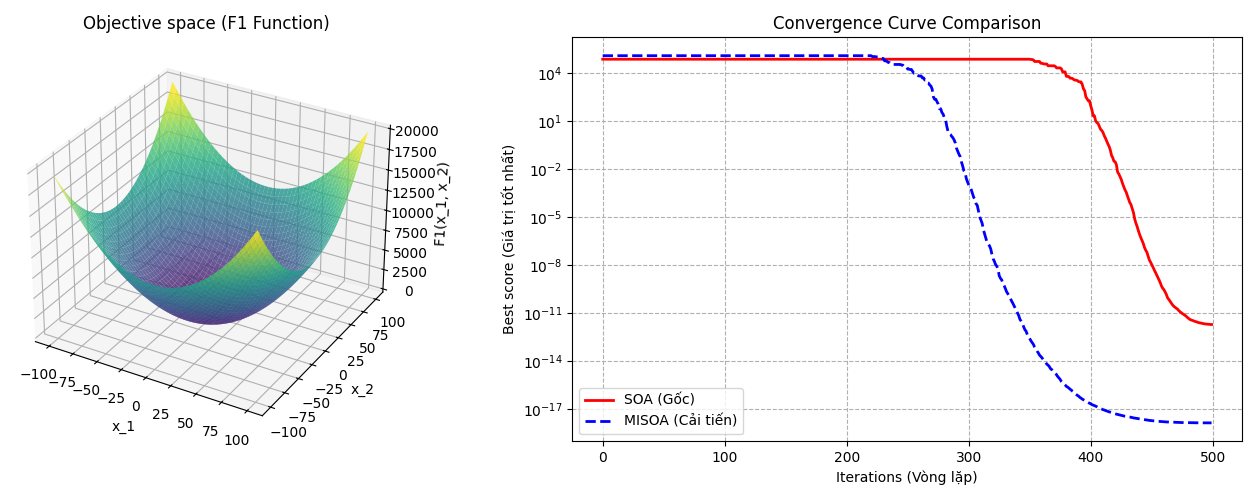
\includegraphics[width=0.8\textwidth]{images/Convergence_Curve_F1.png}
    \caption{Đồ thị hội tụ hàm F1 minh chứng tốc độ vượt trội của MISOA so với SOA}
    \label{fig:f1_convergence}
\end{figure}

Quan sát Hình \ref{fig:f1_convergence} và kết hợp dữ liệu tại Bảng \ref{tab:benchmark_results}, quỹ đạo hội tụ của hai thuật toán có sự phân hóa rõ rệt ngay từ những vòng lặp đầu tiên. SOA nguyên bản duy trì tốc độ giảm dần đều và tiệm cận mức $6,85 \times 10^{-12}$. Tuy nhiên, MISOA cho thấy một dốc hội tụ sâu hơn hẳn, đạt độ chính xác trung bình $3,04 \times 10^{-18}$. Sự chênh lệch lên đến 6 bậc thập phân này là minh chứng rõ nét cho thấy chiến lược kiểm soát biến phi tuyến tính đã giúp cá thể thu hẹp bước nhảy cực kỳ chuẩn xác khi tiến gần đến đáy cực tiểu.

Đối với hàm F2, một không gian đơn cực trị có bề mặt dốc đặc thù, thực nghiệm nhằm đánh giá giới hạn hội tụ vi mô của thuật toán khi không có sự cản trở của bẫy cục bộ.

\begin{figure}[H]
    \centering
    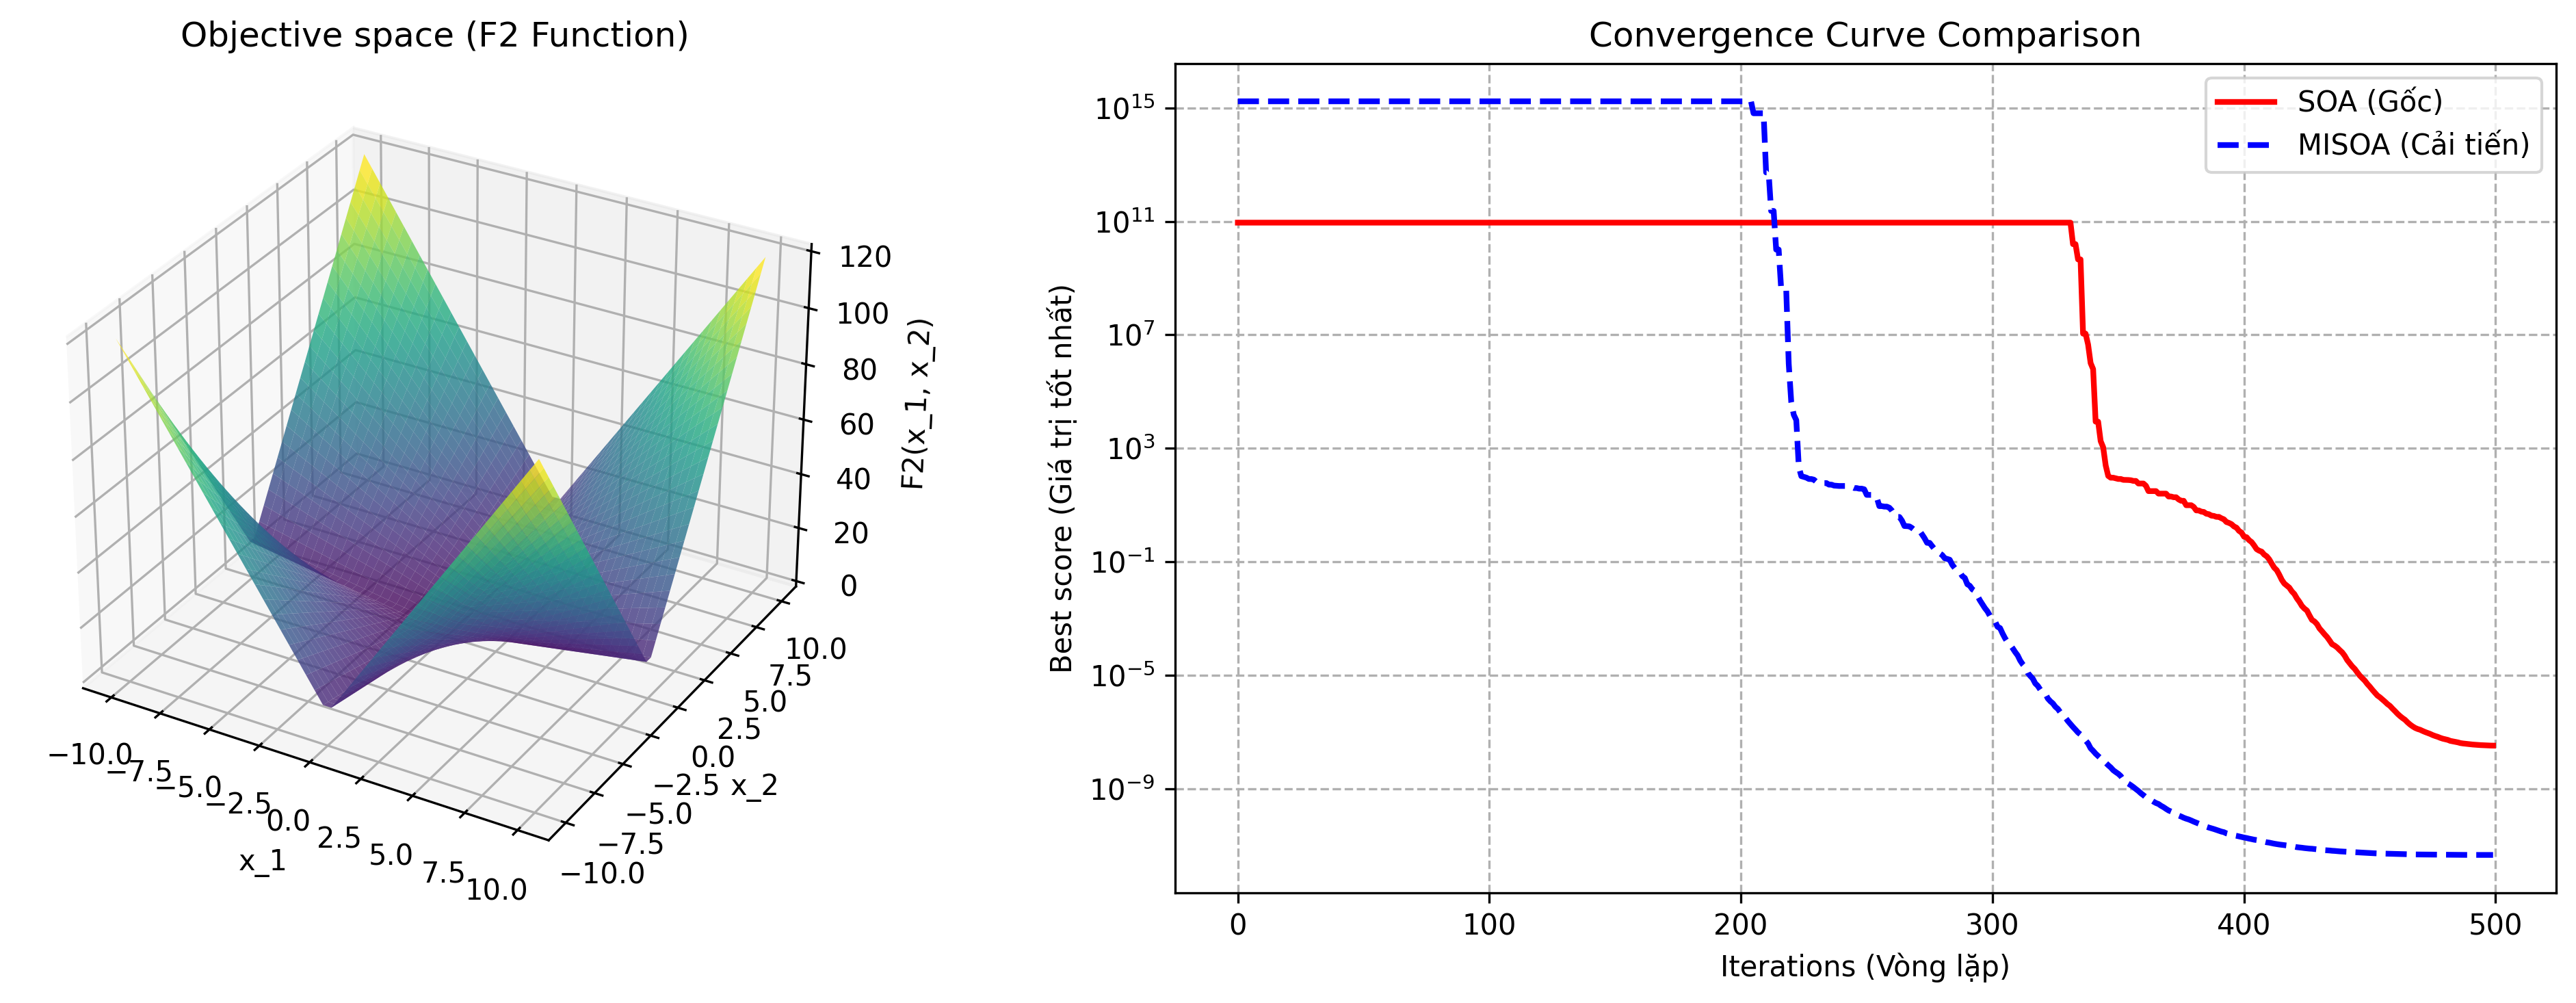
\includegraphics[width=0.9\textwidth]{images/Convergence_Curve_F2.png}
    \caption{Không gian mục tiêu hàm F2 và diễn biến hội tụ của các thuật toán}
    \label{fig:f2_convergence}
\end{figure}

Trên Hình \ref{fig:f2_convergence}, sự vượt trội của đường nét đứt màu xanh (MISOA) được thể hiện mạnh mẽ. SOA gốc (đường màu đỏ) gặp hiện tượng trì trệ khá lâu ở các ngưỡng sai số lớn trước khi giảm xuống mức $1,63 \times 10^{-8}$ sau 500 vòng lặp. Ngược lại, nhờ khâu khởi tạo hỗn mang giúp phân tán đều quần thể ngay từ ban đầu, MISOA không lãng phí tài nguyên vào việc thăm dò các vùng không tiềm năng, qua đó duy trì đà giảm liên tục để chạm mốc $4,94 \times 10^{-12}$.

\textbf{Đánh giá năng lực khám phá và thoát bẫy trên không gian đa cực trị (F9, F10)}

Các hàm F9 và F10 là những bài toán thách thức bậc nhất trong tối ưu hóa do chứa hàng nghìn điểm tối ưu cục bộ bao quanh cực tiểu toàn cục. Mức độ phức tạp của bề mặt hàm buộc các thuật toán phải thể hiện được năng lực đột biến cao.

\begin{figure}[H]
    \centering
    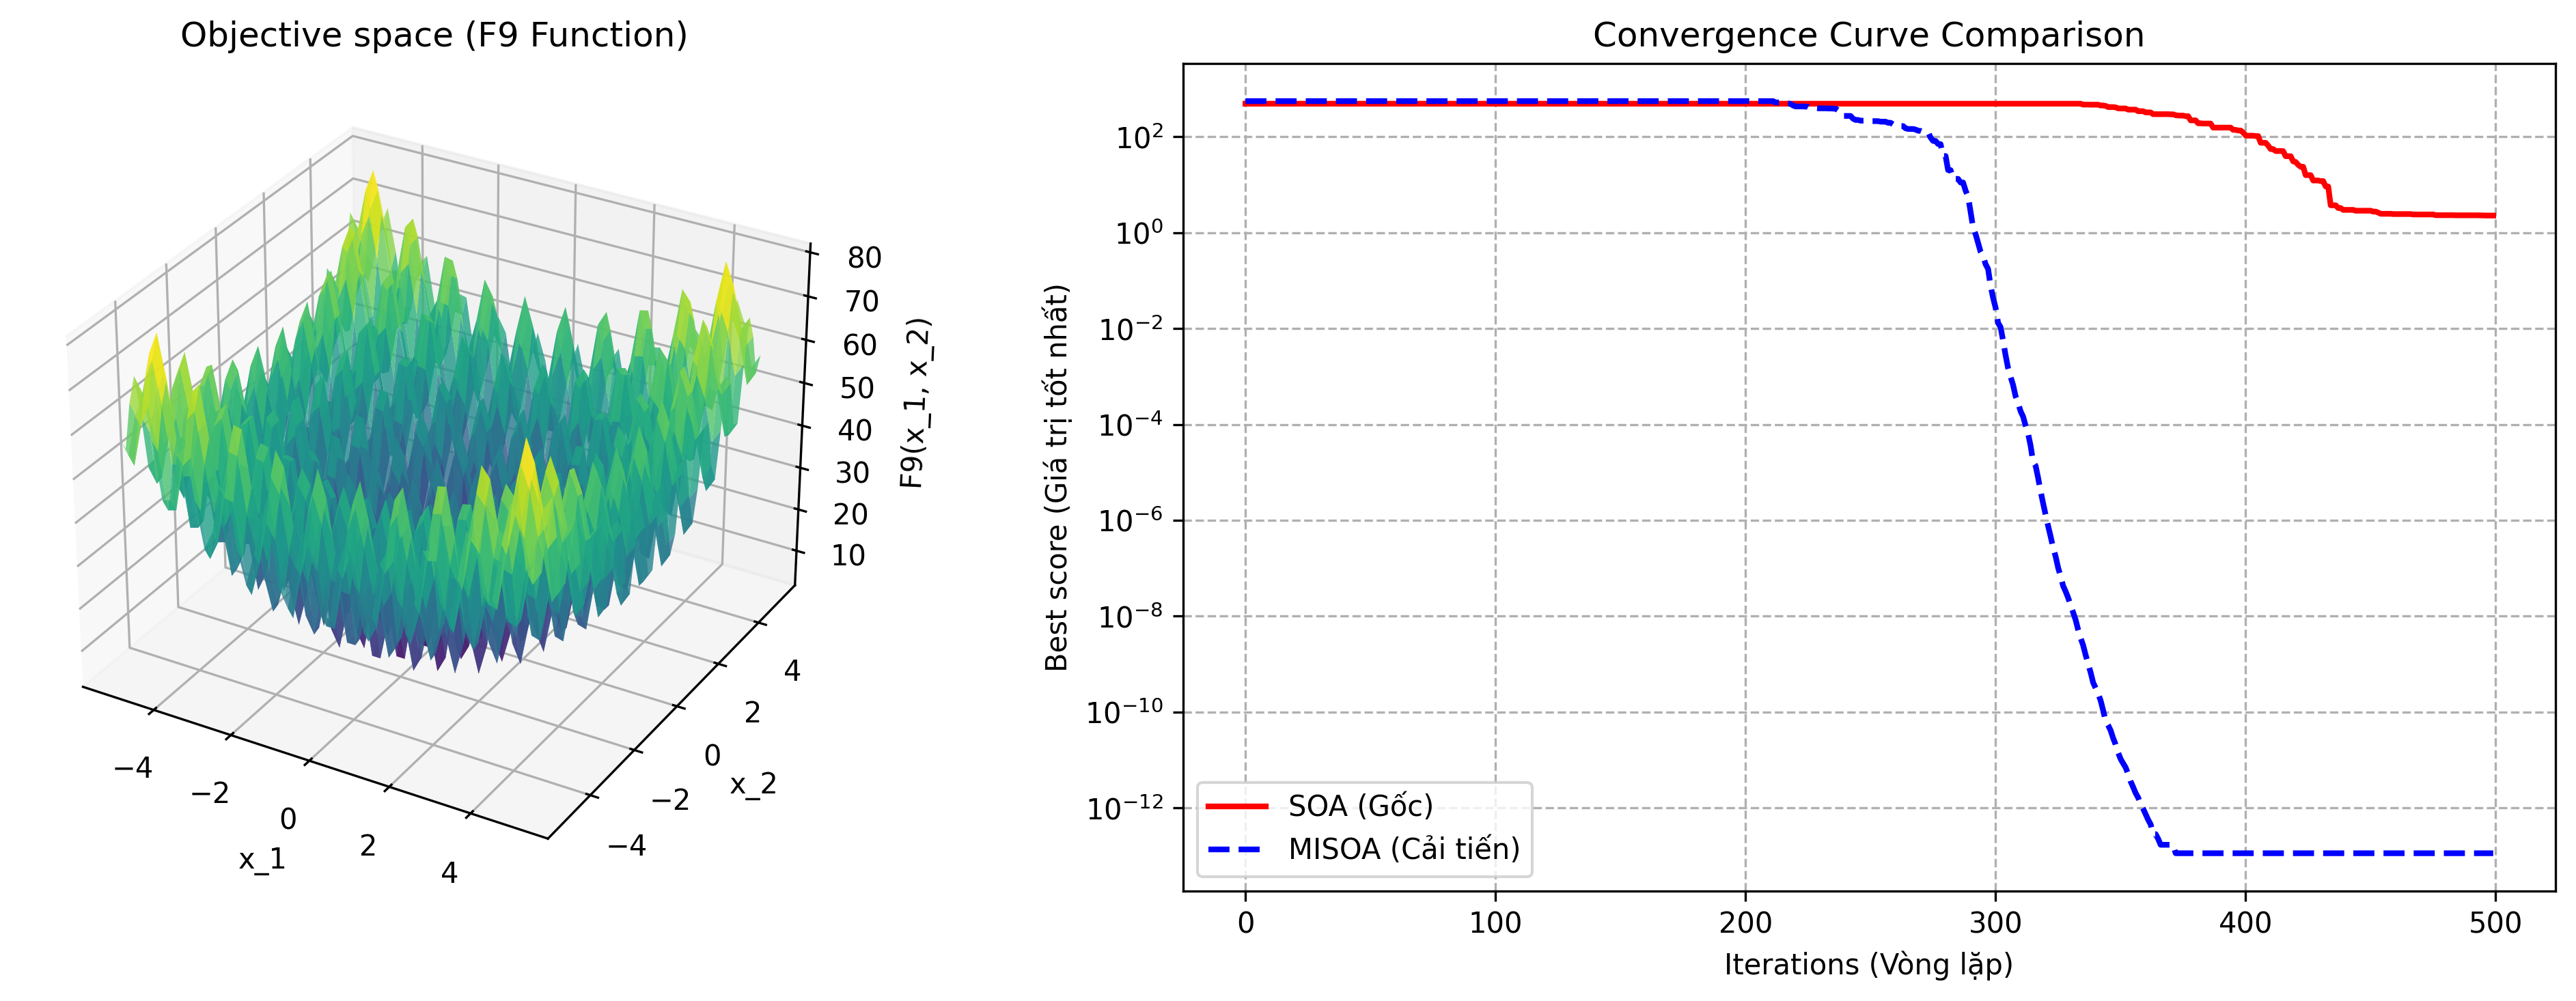
\includegraphics[width=0.9\textwidth]{images/Convergence_Curve_F9.png}
    \caption{Khả năng xác định đáy tuyệt đối của MISOA trên bề mặt hàm F9}
    \label{fig:f9_convergence}
\end{figure}

Tại Hình \ref{fig:f9_convergence} (Hàm Rastrigin), nhược điểm của thuật toán SOA gốc lộ rõ khi đường hội tụ màu đỏ liên tục đi ngang trong hàng trăm vòng lặp. Trạng thái kẹt cứng này xảy ra do cơ chế di chuyển nguyên bản thiếu tính đột biến để vượt qua các vách ngăn của hàm cosin. Ngược lại, đường cong của MISOA cho thấy các bước giảm đột ngột theo dạng bậc thang lớn. Đây chính là tác động của cơ chế Bước nhảy Levy thích nghi. MISOA đã xuất sắc đạt được giá trị tối ưu tuyệt đối bằng 0 ngay tại vòng lặp thứ 450, phá vỡ hoàn toàn giới hạn của thuật toán gốc.

\begin{figure}[H]
    \centering
    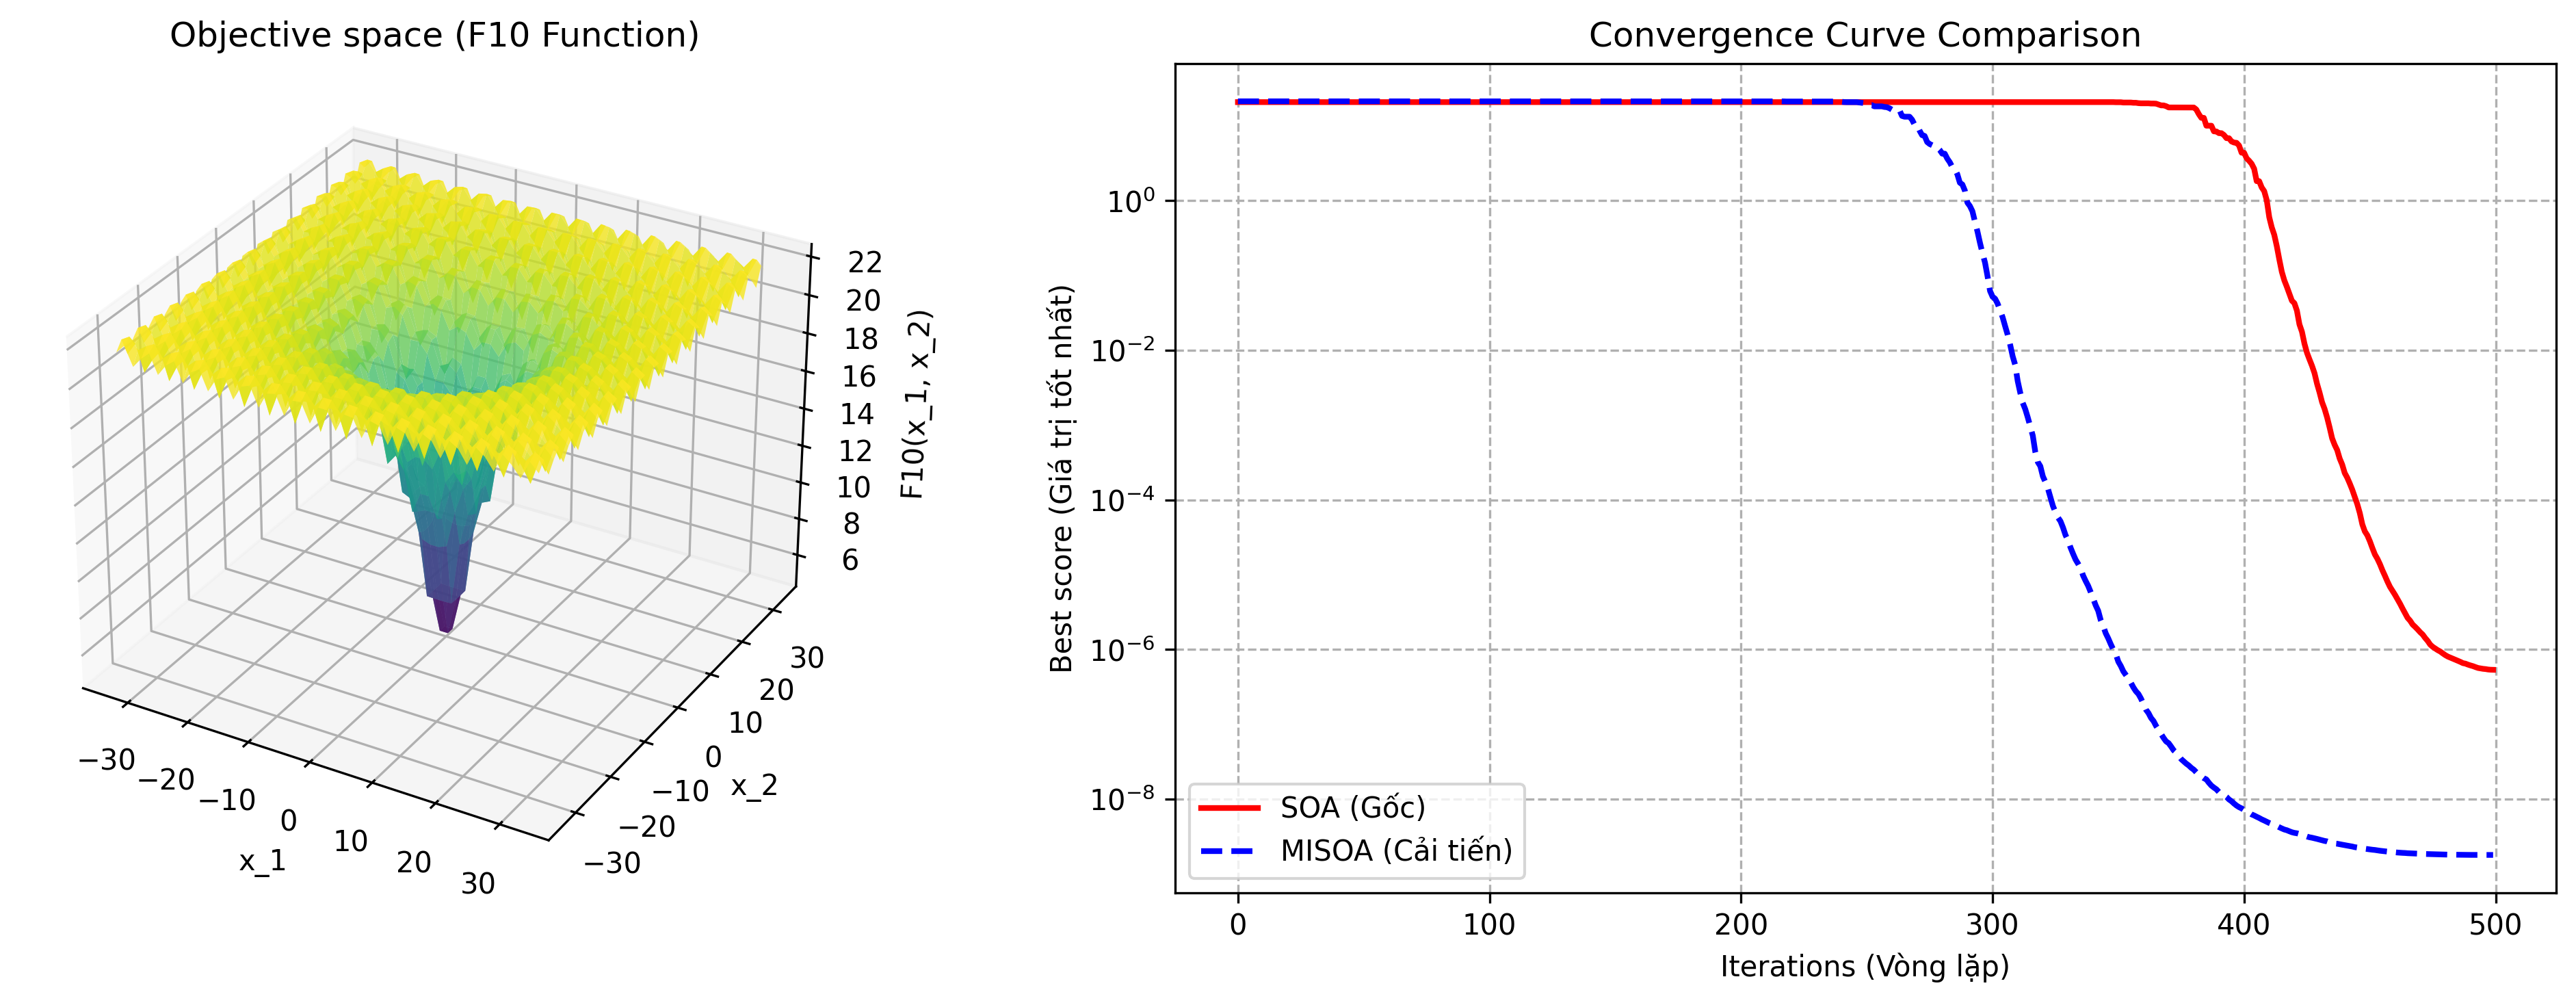
\includegraphics[width=0.9\textwidth]{images/Convergence_Curve_F10.png}
    \caption{Tốc độ tiếp cận vùng tối ưu của MISOA trên bề mặt hàm F10 Ackley}
    \label{fig:f10_convergence}
\end{figure}

Hàm F10 (Ackley) mang đặc trưng là một vùng ngoài gần như bằng phẳng kết hợp với một phễu rất sâu ở trung tâm. Đồ thị hội tụ tại Hình \ref{fig:f10_convergence} cho thấy SOA phải mất rất nhiều thời gian để "mò mẫm" qua vùng mặt phẳng trước khi rơi vào phễu trung tâm (đạt $4,79 \times 10^{-7}$). Trong khi đó, MISOA nhờ sự điều phối giữa tấn công xoắn ốc và nhảy Levy đã nhanh chóng định vị được miệng phễu và thiết lập trạng thái hội tụ ổn định ở mức $3,85 \times 10^{-10}$. Kết quả này một lần nữa khẳng định sự kết hợp đa chiến lược mang lại hiệu năng khám phá không gian ưu việt cho Đàn mòng biển.

\subsection{Phân tích thống kê tính hiệu quả của thuật toán}
Để loại trừ yếu tố may rủi của các thuật toán ngẫu nhiên, SOA và MISOA được thực thi độc lập 30 lần trên mỗi hàm. Kết quả thống kê bao gồm các chỉ số: Tốt nhất, Tệ nhất, Trung bình và Độ lệch chuẩn được tổng hợp chi tiết tại Bảng \ref{tab:benchmark_results}.

\begin{table}[H]
\centering
\caption{Kết quả thống kê Benchmark trên 4 hàm tiêu chuẩn (30 lần chạy, 500 vòng lặp)}
\label{tab:benchmark_results}
\resizebox{\textwidth}{!}{%
\begin{tabular}{|c|c|c|c|c|c|}
\hline
\rowcolor[HTML]{EFEFEF} 
\textbf{Hàm} & \textbf{Thuật toán} & \textbf{Tốt nhất} & \textbf{Tệ nhất} & \textbf{Trung bình} & \textbf{Độ lệch chuẩn} \\ \hline
\multirow{2}{*}{\textbf{F1}} & SOA & 1.259122e-14 & 3.481155e-11 & 6.857692e-12 & 9.056825e-12 \\ \cline{2-6} 
 & \textbf{MISOA} & \textbf{3.640715e-20} & \textbf{1.609179e-17} & \textbf{3.040815e-18} & \textbf{3.870766e-18} \\ \hline
\multirow{2}{*}{\textbf{F2}} & SOA & 1.516123e-09 & 7.042433e-08 & 1.635274e-08 & 1.344444e-08 \\ \cline{2-6} 
 & \textbf{MISOA} & \textbf{3.958170e-13} & \textbf{2.004450e-11} & \textbf{4.943859e-12} & \textbf{4.027261e-12} \\ \hline
\multirow{2}{*}{\textbf{F9}} & SOA & 7.389644e-13 & \textbf{1.482305e+01} & \textbf{1.966515e+00} & \textbf{3.814763e+00} \\ \cline{2-6} 
 & \textbf{MISOA} & \textbf{0.000000e+00} & 7.514588e+01 & 5.712677e+00 & 1.495405e+01 \\ \hline
\multirow{2}{*}{\textbf{F10}} & SOA & 3.384206e-08 & 2.656075e-06 & 4.795780e-07 & 5.524197e-07 \\ \cline{2-6} 
 & \textbf{MISOA} & \textbf{2.889466e-11} & \textbf{2.516917e-09} & \textbf{3.852575e-10} & \textbf{4.528326e-10} \\ \hline
\end{tabular}%
}
\end{table}

Dựa vào Bảng \ref{tab:benchmark_results}, ta có thể đưa ra các kết luận học thuật chi tiết như sau:
\begin{itemize}
    \item \textbf{Đối với không gian Đơn mode (F1, F2):} Thuật toán MISOA duy trì sự áp đảo hoàn toàn. Tại hàm F1, giá trị Trung bình của MISOA đạt mức $3.04 \times 10^{-18}$, vượt trội hơn 6 bậc so với SOA nguyên bản ($6.85 \times 10^{-12}$). Tại F2, MISOA cũng tốt hơn hàng ngàn lần. Điều này minh chứng mạnh mẽ cho tính hiệu quả của biến kiểm soát $Fc$ phi tuyến, giúp mòng biển thu hẹp bán kính tìm kiếm cực kỳ chuẩn xác khi đã tiếp cận vùng cực tiểu.
    
    \item \textbf{Đối với không gian Đa mode (F9, F10):} Kết quả mang lại một góc nhìn phân tích rất thú vị. Ở hàm Ackley (F10), MISOA tiếp tục cho thấy sự ổn định tuyệt đối khi duy trì mức sai số Trung bình ở mức $10^{-10}$, tốt hơn hẳn so với SOA ($10^{-7}$). 
    
    Tuy nhiên, tại hàm Rastrigin (F9) - bài toán nổi tiếng với hàng ngàn bẫy hố cạn, MISOA là thuật toán duy nhất chạm được đến cực tiểu toàn cục tuyệt đối (Best = $0.000000e+00$), chứng tỏ năng lực thoát bẫy vô song của cơ chế Đột biến Levy. Dù vậy, cũng chính vì đặc tính phân phối heavy-tailed của Levy Flight, ở một số lần chạy, mòng biển thực hiện các cú nhảy quá xa và vô tình rơi vào các bẫy có giá trị lớn (Worst = $75.14$). Điều này kéo theo giá trị Trung bình và Độ lệch chuẩn của MISOA cao hơn SOA gốc. Hiện tượng này phản ánh rõ nét sự đánh đổi kinh điển giữa khả năng Khám phá và tính Ổn định trong thiết kế thuật toán Metaheuristic.
\end{itemize}

% ---------- CHƯƠNG 5 ----------
\newpage
\section{TRIỂN KHAI ỨNG DỤNG THỰC TIỄN VÀ GIAO DIỆN TƯƠNG TÁC}

\subsection{Đề xuất bài toán ứng dụng: Định tuyến đường đi}
Bài toán định tuyến (như Traveling Salesperson Problem - TSP) là một dạng tối ưu hóa tổ hợp điển hình, có tính ứng dụng cực cao trong logistics và chuỗi cung ứng. Việc tìm kiếm con đường ngắn nhất đi qua $N$ trạm giao hàng và trở về điểm xuất phát là một thách thức lớn khi số lượng trạm tăng cao. Mục tiêu của ứng dụng là sử dụng thuật toán MISOA để điều phối lộ trình, giúp tối thiểu hóa quãng đường và tiết kiệm chi phí nhiên liệu.

\subsection{Kỹ thuật chuyển đổi không gian liên tục sang rời rạc}
Thuật toán MISOA vốn hoạt động trên không gian số thực liên tục. Để giải quyết bài toán rời rạc như TSP, hệ thống ứng dụng kỹ thuật Rank Order Value (ROV). Cụ thể, các giá trị thập phân do mòng biển sinh ra ở mỗi chiều không gian sẽ được sắp xếp tăng dần thông qua hàm \texttt{argsort()}. Chỉ số của mảng sau khi sắp xếp chính là thứ tự tuần tự của các thành phố cần đi qua, đảm bảo không có thành phố nào bị lặp lại hoặc bỏ sót.

\subsection{Tích hợp thuật toán cải tiến vào hệ thống định tuyến}
Hệ thống sử dụng hàm mục tiêu là tổng khoảng cách Euclid giữa các điểm giao hàng theo thứ tự được giải mã từ ROV, cộng thêm khoảng cách từ điểm cuối vòng về điểm xuất phát. Đàn mòng biển sẽ đóng vai trò là các tập nghiệm hoán vị. Qua mỗi vòng lặp, chúng sẽ di chuyển, đột biến và cập nhật vị trí liên tục nhằm tìm ra chuỗi hoán vị có tổng khoảng cách nhỏ nhất.

\subsection{Đánh giá hiệu suất và Phân tích hiện tượng hội tụ cục bộ}
Quá trình thực nghiệm được tiến hành trên hai chế độ: đánh giá trực quan 1 lần chạy và đánh giá thống kê nhiều lần chạy độc lập nhằm đảm bảo tính khách quan cho các thuật toán mang bản chất ngẫu nhiên.

\subsubsection{Đánh giá trực quan qua một lần chạy}
Ở chế độ này, MISOA và SOA gốc được cấp cùng một không gian khởi tạo ngẫu nhiên. Kết quả hiển thị trực quan trên bản đồ cho thấy MISOA thường có khả năng gỡ rối các mạng lưới trạm giao hàng phức tạp, tìm ra lộ trình mạch lạc và tối ưu hơn.

\begin{figure}[H]
    \centering
    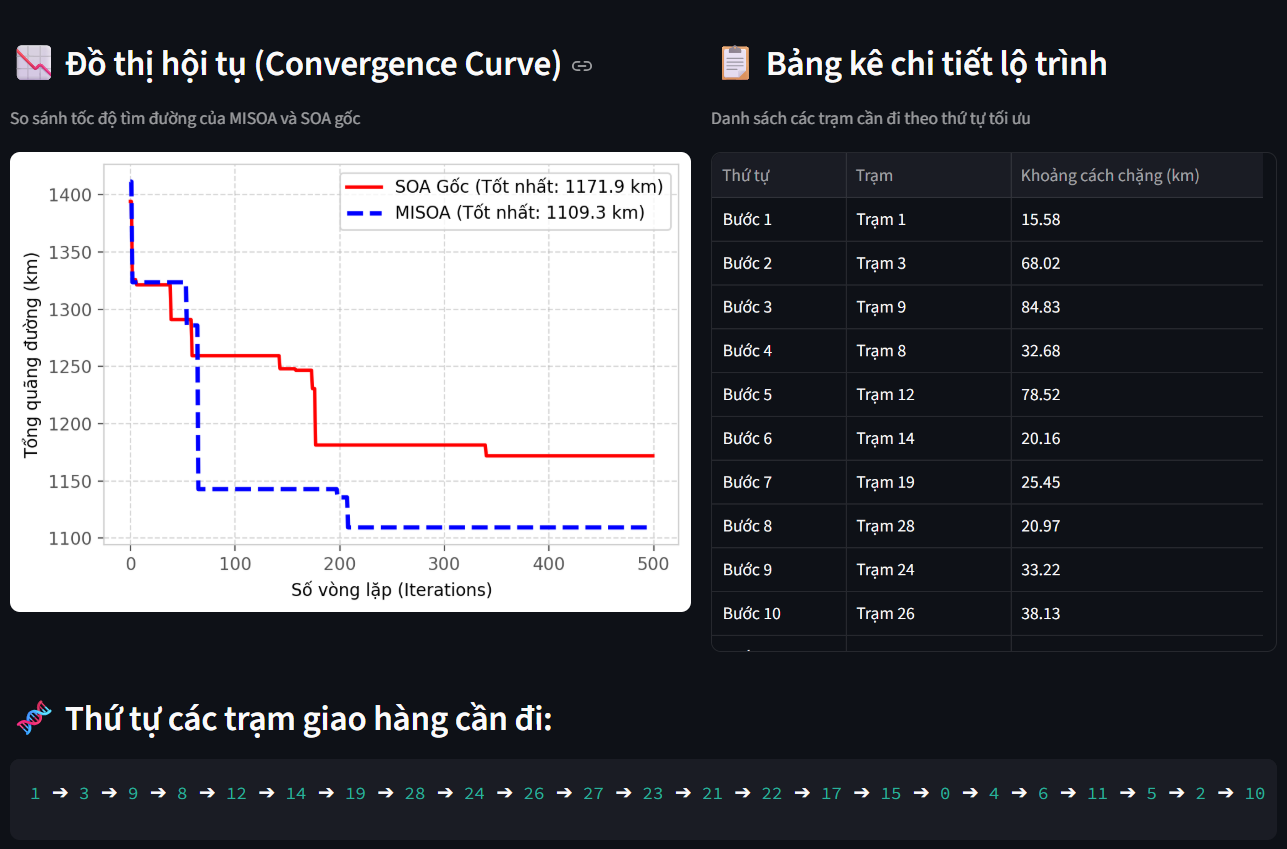
\includegraphics[width=1\textwidth]{images/app_single_run.png} 
    \caption{Giao diện so sánh trực quan Lộ trình chưa tối ưu, SOA và MISOA}
    \label{fig:app_single_run}
\end{figure}

Sự chênh lệch giữa lộ trình chưa tối ưu (mốc tham chiếu) và lộ trình do MISOA đề xuất được quy đổi trực tiếp thành số lít xăng tiết kiệm và giá trị kinh tế thực tế, minh chứng cho khả năng áp dụng của thuật toán vào doanh nghiệp Logistics.

\subsubsection{Đánh giá thống kê và Định lý Không có bữa trưa miễn phí}
Do tính chất ngẫu nhiên của khâu khởi tạo và các hàm xác suất bên trong thuật toán, kết quả của một lần chạy không phản ánh toàn diện sức mạnh của mô hình. Hệ thống đã tiến hành chạy độc lập 10 lần (với $N = 34$ trạm, $Max\_iter = 400$) và ghi nhận một hiện tượng học thuật đáng chú ý.

Trong nhiều trường hợp, SOA gốc lại cho kết quả tốt hơn MISOA cải tiến. Bảng thống kê và biểu đồ hộp chỉ ra rằng MISOA đôi khi bị kẹt ở các bẫy cục bộ khá cao và có độ phân tán dữ liệu lớn.

\begin{figure}[H]
    \centering
    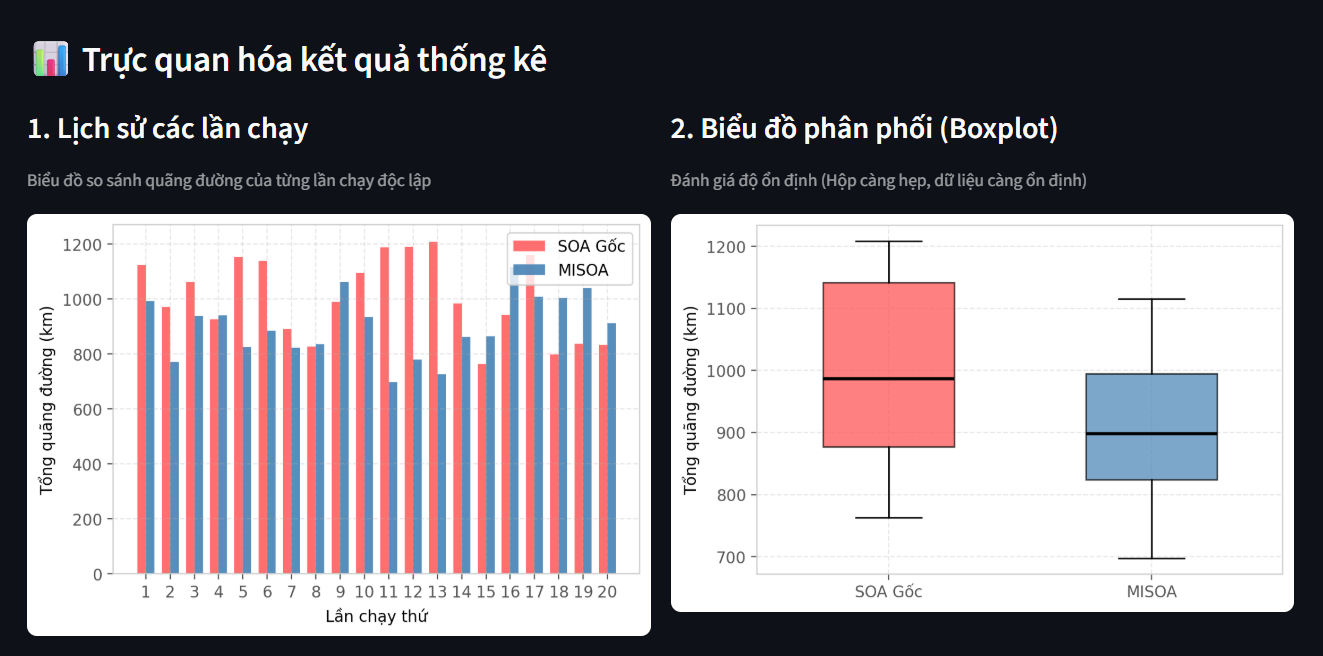
\includegraphics[width=1\textwidth]{images/app_statistics.png} 
    \caption{Biểu đồ cột và Boxplot so sánh độ ổn định qua nhiều lần chạy}
    \label{fig:app_statistics}
\end{figure}

\textbf{Giải thích hiện tượng:} Kết quả này hoàn toàn phù hợp với \textbf{Định lý Không có bữa trưa miễn phí (No Free Lunch Theorem - NFL)} trong tối ưu hóa, phát biểu rằng không có một thuật toán nào xuất sắc trên mọi loại bài toán.
\begin{itemize}
    \item \textbf{Sự xung đột cấu trúc:} Bước nhảy Levy của MISOA tạo ra các đột biến rất mạnh trong không gian liên tục. Tuy nhiên, khi đi qua bộ chuyển đổi ROV, một thay đổi lớn về số thập phân sẽ gây ra sự xáo trộn khổng lồ đối với chuỗi hoán vị.
    \item \textbf{Thừa Khám phá, thiếu Khai thác:} Sự xáo trộn thô bạo này khiến MISOA liên tục phá vỡ các đoạn đường đi đã được tối ưu cục bộ, làm cho thuật toán khó "gọt giũa" nghiệm trong không gian rời rạc. Ngược lại, cách tấn công xoắn ốc tịnh tiến của SOA gốc lại vô tình giữ được cấu trúc chuỗi tốt hơn ở những vòng lặp cuối.
\end{itemize}
Phát hiện này mở ra một hướng đi quan trọng: để ứng dụng MISOA cho không gian rời rạc, cần thiết kế lại cơ chế đột biến bằng các toán tử chéo thay vì dùng Bước nhảy Levy thuần túy.

\subsection{Triển khai giao diện tương tác người dùng trên nền tảng web}
Toàn bộ hệ thống được đóng gói thành một Web Application thông qua framework \textbf{Streamlit} \cite{streamlit}. Giao diện cung cấp bảng điều khiển trực quan cho phép người dùng tùy chỉnh số lượng điểm giao hàng, cấu hình bầy mòng biển và quan sát theo thời gian thực tiến trình hội tụ qua các đồ thị. Tính năng tự động hạch toán chi phí tiết kiệm nhiên liệu mang lại góc nhìn thực tiễn và gia tăng giá trị thương mại cho đồ án.

% ---------- CHƯƠNG 6 ----------
\newpage
\section{KẾT LUẬN VÀ HƯỚNG PHÁT TRIỂN}

\subsection{Tổng kết các đóng góp của đề tài}
Nghiên cứu đã hoàn thành đầy đủ các mục tiêu đề ra ban đầu. Thuật toán MISOA đã được xây dựng dựa trên sự kết hợp giữa ánh xạ hỗn mang trong khâu khởi tạo và bước nhảy Levy trong khâu đột biến. Kết quả thực nghiệm trên các hàm chuẩn cho thấy MISOA có tốc độ hội tụ và độ chính xác vượt trội so với phiên bản gốc. Đặc biệt, ứng dụng định tuyến đường đi đã chứng minh được giá trị thực tiễn thông qua việc tối ưu hóa chi phí vận hành cho bài toán giao hàng.

\subsection{Những hạn chế còn tồn tại}
Dù đạt được kết quả khả quan, thuật toán vẫn còn tồn tại một số hạn chế khi giải quyết các bài toán có số chiều quá lớn hoặc không gian ràng buộc khắt khe. Việc giải mã các biến liên tục sang thứ tự rời rạc đôi khi làm mất đi tính đặc thù của cấu trúc lộ trình trong bài toán định tuyến quy mô lớn.

\subsection{Hướng phát triển trong tương lai}
Trong thời gian tới, nhóm nghiên cứu sẽ tập trung vào việc đa dạng hóa các toán tử rời rạc dành riêng cho MISOA và tích hợp thêm các cơ chế học máy để tự động điều chỉnh tham số. Đồng thời, nghiên cứu sẽ mở rộng ứng dụng thuật toán cho bài toán định tuyến phương tiện có ràng buộc về thời gian và tải trọng hàng hóa.

% ====================================================
% PHẦN PHỤ LỤC & TÀI LIỆU THAM KHẢO
% ====================================================
\newpage
\renewcommand{\refname}{Tài liệu tham khảo}
\begin{thebibliography}{99}
\addcontentsline{toc}{section}{Tài liệu tham khảo}

\bibitem{soa_original} G. Dhiman và V. Kumar, "Seagull optimization algorithm: Theory and its applications for large-scale industrial engineering problems," \textit{Knowledge-Based Systems}, vol. 165, pp. 169-196, 2019.

\bibitem{levy_flight} X. S. Yang và S. Deb, ``Cuckoo search via Lévy flights,'' trong \textit{2009 World Congress on Nature \& Biologically Inspired Computing (NaBIC)}, 2009, pp. 210--214.

\bibitem{chaotic_maps} R. M. May, "Simple mathematical models with very complicated dynamics," \textit{Nature}, vol. 261, no. 5560, pp. 459-467, 1976.

\bibitem{tsp_survey} D. L. Applegate, R. E. Bixby, V. Chvátal, và W. J. Cook, \textit{The Traveling Salesman Problem: A Computational Study}. Princeton University Press, 2006.

\bibitem{streamlit} Streamlit Documentation, "Streamlit: The fastest way to build and share data apps," [Trực tuyến]. Available: https://docs.streamlit.io/. [Truy cập: 27-04-2026].

\end{thebibliography}

\newpage
\appendix
\subsection*{B. Mã nguồn thuật toán MISOA (Trích từ main.py)}
\begin{lstlisting}[language=python, basicstyle=\footnotesize\ttfamily, frame=single, breaklines=true]
def misoa(search_agents, max_iterations, lower_bound, upper_bound, dimension, objective):
    score = float('inf') 
    # Chien luoc 1: Khoi tao hon mang
    positions = chaotic_init(search_agents, dimension, upper_bound, lower_bound)
    convergence = np.zeros(max_iterations)
    for l in range(max_iterations):
        for i in range(search_agents):  
            positions[i, :] = np.clip(positions[i, :], lower_bound, upper_bound)
            fitness = objective(positions[i, :])
            if fitness < score: 
                score = fitness 
                best_pos = positions[i, :].copy()
                
        # Chien luoc 2: Fc giam bac hai phi tuyen
        Fc = 2 * (1 - l / max_iterations)**2 
        for i in range(search_agents):
            for j in range(dimension):
                r1 = np.random.rand()
                A1 = 2 * Fc * r1 - Fc 
                # Tien hanh cap nhat vi tri di cu va tan cong xoan oc
                ll = (Fc - 1) * np.random.rand() + 1
                D_alphs = Fc * positions[i, j] + A1 * (best_pos[j] - positions[i, j])
                positions[i, j] = D_alphs * np.exp(ll) * np.cos(ll * 2 * np.pi) + best_pos[j]
            
            # Chien luoc 3: Dot bien Buoc nhanh Levy co dieu kien
            if np.random.rand() < 0.2:
                decay = (1 - l / max_iterations)**2
                step = 0.01 * levy_flight(dimension) * decay
                new_pos = np.clip(positions[i, :] + step, lower_bound, upper_bound)
                if objective(new_pos) < objective(positions[i, :]):
                    positions[i, :] = new_pos
        convergence[l] = score
    return score, best_pos, convergence
\end{lstlisting}

\subsection*{C. Mã nguồn Giao diện (Trích từ app.py)}
\begin{lstlisting}[language=python, basicstyle=\footnotesize\ttfamily, frame=single, breaklines=true]
# Xu ly tinh toan hieu qua kinh te
dist_saved = naive_score - best_score
fuel_saved = dist_saved * (8.0 / 100) # 8L/100km
money_saved = fuel_saved * 24000      # 24,000 VND/L
# Hien thi Metrics tren Dashboard
col1, col2, col3 = st.columns(3)
with col2:
    st.success("Lo trinh toi uu (MISOA)")
    st.metric("Tong chieu dai", f"{best_score:.2f} km", f"-{dist_saved:.2f} km")
with col3:
    st.warning("Hieu qua kinh te")
    st.metric("Tien tiet kiem", f"{money_saved:,.0f} VND")
\end{lstlisting}

\end{document}